% Options for packages loaded elsewhere
\PassOptionsToPackage{unicode}{hyperref}
\PassOptionsToPackage{hyphens}{url}
\PassOptionsToPackage{dvipsnames,svgnames,x11names}{xcolor}
%
\documentclass[
  11pt,
]{article}

\usepackage{amsmath,amssymb}
\usepackage{iftex}
\ifPDFTeX
  \usepackage[T1]{fontenc}
  \usepackage[utf8]{inputenc}
  \usepackage{textcomp} % provide euro and other symbols
\else % if luatex or xetex
  \usepackage{unicode-math}
  \defaultfontfeatures{Scale=MatchLowercase}
  \defaultfontfeatures[\rmfamily]{Ligatures=TeX,Scale=1}
\fi
\usepackage{lmodern}
\ifPDFTeX\else  
    % xetex/luatex font selection
\fi
% Use upquote if available, for straight quotes in verbatim environments
\IfFileExists{upquote.sty}{\usepackage{upquote}}{}
\IfFileExists{microtype.sty}{% use microtype if available
  \usepackage[]{microtype}
  \UseMicrotypeSet[protrusion]{basicmath} % disable protrusion for tt fonts
}{}
\makeatletter
\@ifundefined{KOMAClassName}{% if non-KOMA class
  \IfFileExists{parskip.sty}{%
    \usepackage{parskip}
  }{% else
    \setlength{\parindent}{0pt}
    \setlength{\parskip}{6pt plus 2pt minus 1pt}}
}{% if KOMA class
  \KOMAoptions{parskip=half}}
\makeatother
\usepackage{xcolor}
\usepackage[left=2.54cm,right=2.54cm]{geometry}
\setlength{\emergencystretch}{3em} % prevent overfull lines
\setcounter{secnumdepth}{5}
% Make \paragraph and \subparagraph free-standing
\ifx\paragraph\undefined\else
  \let\oldparagraph\paragraph
  \renewcommand{\paragraph}[1]{\oldparagraph{#1}\mbox{}}
\fi
\ifx\subparagraph\undefined\else
  \let\oldsubparagraph\subparagraph
  \renewcommand{\subparagraph}[1]{\oldsubparagraph{#1}\mbox{}}
\fi


\providecommand{\tightlist}{%
  \setlength{\itemsep}{0pt}\setlength{\parskip}{0pt}}\usepackage{longtable,booktabs,array}
\usepackage{calc} % for calculating minipage widths
% Correct order of tables after \paragraph or \subparagraph
\usepackage{etoolbox}
\makeatletter
\patchcmd\longtable{\par}{\if@noskipsec\mbox{}\fi\par}{}{}
\makeatother
% Allow footnotes in longtable head/foot
\IfFileExists{footnotehyper.sty}{\usepackage{footnotehyper}}{\usepackage{footnote}}
\makesavenoteenv{longtable}
\usepackage{graphicx}
\makeatletter
\def\maxwidth{\ifdim\Gin@nat@width>\linewidth\linewidth\else\Gin@nat@width\fi}
\def\maxheight{\ifdim\Gin@nat@height>\textheight\textheight\else\Gin@nat@height\fi}
\makeatother
% Scale images if necessary, so that they will not overflow the page
% margins by default, and it is still possible to overwrite the defaults
% using explicit options in \includegraphics[width, height, ...]{}
\setkeys{Gin}{width=\maxwidth,height=\maxheight,keepaspectratio}
% Set default figure placement to htbp
\makeatletter
\def\fps@figure{htbp}
\makeatother
\newlength{\cslhangindent}
\setlength{\cslhangindent}{1.5em}
\newlength{\csllabelwidth}
\setlength{\csllabelwidth}{3em}
\newlength{\cslentryspacingunit} % times entry-spacing
\setlength{\cslentryspacingunit}{\parskip}
\newenvironment{CSLReferences}[2] % #1 hanging-ident, #2 entry spacing
 {% don't indent paragraphs
  \setlength{\parindent}{0pt}
  % turn on hanging indent if param 1 is 1
  \ifodd #1
  \let\oldpar\par
  \def\par{\hangindent=\cslhangindent\oldpar}
  \fi
  % set entry spacing
  \setlength{\parskip}{#2\cslentryspacingunit}
 }%
 {}
\usepackage{calc}
\newcommand{\CSLBlock}[1]{#1\hfill\break}
\newcommand{\CSLLeftMargin}[1]{\parbox[t]{\csllabelwidth}{#1}}
\newcommand{\CSLRightInline}[1]{\parbox[t]{\linewidth - \csllabelwidth}{#1}\break}
\newcommand{\CSLIndent}[1]{\hspace{\cslhangindent}#1}

\usepackage[noblocks]{authblk}
\renewcommand*{\Authsep}{, }
\renewcommand*{\Authand}{, }
\renewcommand*{\Authands}{, }
\renewcommand\Affilfont{\small}
\usepackage{lipsum} \usepackage{libertine}
\makeatletter
\makeatother
\makeatletter
\makeatother
\makeatletter
\@ifpackageloaded{caption}{}{\usepackage{caption}}
\AtBeginDocument{%
\ifdefined\contentsname
  \renewcommand*\contentsname{Table of contents}
\else
  \newcommand\contentsname{Table of contents}
\fi
\ifdefined\listfigurename
  \renewcommand*\listfigurename{List of Figures}
\else
  \newcommand\listfigurename{List of Figures}
\fi
\ifdefined\listtablename
  \renewcommand*\listtablename{List of Tables}
\else
  \newcommand\listtablename{List of Tables}
\fi
\ifdefined\figurename
  \renewcommand*\figurename{Figure}
\else
  \newcommand\figurename{Figure}
\fi
\ifdefined\tablename
  \renewcommand*\tablename{Table}
\else
  \newcommand\tablename{Table}
\fi
}
\@ifpackageloaded{float}{}{\usepackage{float}}
\floatstyle{ruled}
\@ifundefined{c@chapter}{\newfloat{codelisting}{h}{lop}}{\newfloat{codelisting}{h}{lop}[chapter]}
\floatname{codelisting}{Listing}
\newcommand*\listoflistings{\listof{codelisting}{List of Listings}}
\makeatother
\makeatletter
\@ifpackageloaded{caption}{}{\usepackage{caption}}
\@ifpackageloaded{subcaption}{}{\usepackage{subcaption}}
\makeatother
\makeatletter
\@ifpackageloaded{tcolorbox}{}{\usepackage[skins,breakable]{tcolorbox}}
\makeatother
\makeatletter
\@ifundefined{shadecolor}{\definecolor{shadecolor}{rgb}{.97, .97, .97}}
\makeatother
\makeatletter
\makeatother
\makeatletter
\makeatother
\ifLuaTeX
  \usepackage{selnolig}  % disable illegal ligatures
\fi
\IfFileExists{bookmark.sty}{\usepackage{bookmark}}{\usepackage{hyperref}}
\IfFileExists{xurl.sty}{\usepackage{xurl}}{} % add URL line breaks if available
\urlstyle{same} % disable monospaced font for URLs
\hypersetup{
  pdftitle={Urban mobility and socioeconomic deprivation in Latin America after COVID-19},
  pdfauthor={Carmen Cabrera-Arnau; Francisco Rowe; Miguel González-Leonardo; Andrea Nasuto; Ruth Neville},
  colorlinks=true,
  linkcolor={blue},
  filecolor={Maroon},
  citecolor={Blue},
  urlcolor={Blue},
  pdfcreator={LaTeX via pandoc}}

\title{\textbf{Urban mobility and socioeconomic deprivation in Latin
America after COVID-19}}


\author[1]{Carmen Cabrera-Arnau}
\author[1]{Francisco Rowe}
\author[2]{Miguel González-Leonardo}
\author[1]{Andrea Nasuto}
\author[1]{Ruth Neville}

\affil[1]{Geographic Data Science Lab, Department of Geography and
Planning, University of Liverpool, Liverpool, UK}
\affil[2]{Centre for Demographic Urban and Environmental Studies, El
Colegio de México, Ciudad de México, México}


\date{}
\begin{document}
\maketitle
\begin{abstract}
The movement of people between locations is crucial for sustainable and
inclusive cities, facilitating the exchange of knowledge and resources.
Due to restrictions, lockdowns and fear of crowded places, the COVID-19
pandemic significantly reduced the number and extent of people's
movements. Existing research suggests that the impact of the pandemic on
mobility was unequal across locations and socioeconomic groups. However,
evidence and analysis of long-term changes in mobility is scarce,
especially in less developed countries. In this study, we use location
data from Meta-Facebook users to analyse patterns of urban mobility in X
Functional Urban Areas from South American countries. Findings reveal a
general decrease in mobility during the pandemic, with gradual recovery
trends up to April 2023. However, socioeconomic disparities are present
through the period of analysis, with deprived areas experiencing smaller
initial losses in mobility. These disparities generally diminish over
time, although they persist in all the countries included in the
analysis. Our research highlights the importance of timely mobility data
with high spatiotemporal resolution to understand the long-term effects
of the pandemic and to inform equitable policy responses that address
societal challenges in urban areas.
\end{abstract}
\ifdefined\Shaded\renewenvironment{Shaded}{\begin{tcolorbox}[boxrule=0pt, frame hidden, breakable, enhanced, interior hidden, sharp corners, borderline west={3pt}{0pt}{shadecolor}]}{\end{tcolorbox}}\fi

\hypertarget{sec-intro}{%
\section{Introduction}\label{sec-intro}}

Spatial human mobility is key to creating sustainable, livable and
inclusive cities. At the societal level, spatial mobility enables the
transfer of knowledge, skills and labour to places they are needed.
Spatial mobility also shapes service and transport demand across urban
spaces, and enables the monitoring and control of transmissible
diseases. At the individual level, mobility enables people to access and
achieve opportunities and aspirations in space. Understanding spatial
human mobility is thus important to supporting appropriate policy
responses to address societal challenges relating to carbon emissions,
urban planning, service delivery, public health, disaster management and
transport.

The COVID-19 pandemic resulted in a notable decrease in mobility,
particularly in cities. This decrease in the overall levels of mobility
was prompted by nonpharmaceutical interventions to contain the spread of
COVID‐19, coupled with general fears of visiting crowded public
spaces.Especially during lockdowns, mobility recorded reductions in the
frequency, distance and time of trips in cities across the globe. Higher
engagement with remote working, online schooling and shopping activity
reduced the need to travel for work, education, shopping and leisure,
hence giving rise to more geographically localised mobility patterns.

However, reductions in mobility levels were highly unequal reflecting
existing socioeconomic inequalities. In most countries, affluent
individuals tended to record the greatest drops in mobility levels as
they are predominantly employed in knowledge-intensive jobs which can be
done fully or partly remotely. During the COVID-19 pandemic, the
adoption of remote work reduced the need of commuting for
knowledge-intensive, non-public facing jobs. At the same time,
individuals from less privileged socioeconomic backgrounds displayed
less pronounced declines mirroring the nature of their work requiring
public-facing, face-to-face interaction, and thus a requirement for
daily work commutes.

Thus, while a growing body of empirical evidence has contributed to
advancing our understanding of the impacts of the COVID-19 pandemic on
spatial mobility within cities, existing research has focused on more
developed countries and the immediate effects of the pandemic during
2020. Less is known about the longer term patterns of resilience in
urban mobility in less developed countries. Assessing the extent to
which the level of mobility has returned back to the pre-pandemic
baseline level across socioeconomic groups is important to understand
the potentially unequal impacts of hybrid working in the society.

A key barrier to monitor changes in geographic mobility patterns in less
developed countries during and post the COVID-19 pandemic has been the
lack of suitable data. Traditionally census and survey data have been
employed to analyse human mobility patterns in these countries. Yet,
these data streams are not frequently updated and suffer from slow
releases, with census data for example being collected over intervals of
ten years in most countries. Traditional data streams thus lack the
temporal granularity to analyse population movements over short-time
periods and to offer an up-to-date representation of the urban mobility
system. Data resulting from social interactions on digital platforms
have emerged as an unique source of information to deliver this
representation and capture human population movement in less developed
countries at scale. Particularly location data from mobile phone
applications have become a prominent source to sense patterns of human
mobility at higher geographical and temporal resolution in real time.

Drawing on a dataset of 213 million observations from Meta-Facebook
users' mobile location data, we aim to assess socioeconomic differences
in the extent and persistence of decline in urban mobility in Argentina,
Chile, Colombia and Mexico during and after the COVID-19 pandemic from
March 2020 to March 2023. We use Meta-Facebook data to measure
origin-destination flows from March 2020 to May 2022, and Meta Prophet
time-series forecasting machine learning algorithm to predict
origin-destination flows from June 2022 to March 2023. We use Functional
Urban Areas (FUAs) boundaries from the Global Human Settlement Layer
(GHSL), developed by the European Comission's Joint Research Centre
(Schiavina M. 2019) to define urban areas; and the Global Gridded
Relative Deprivation Index (GRDI) developed by NASA's Socioeconomic Data
and Applications Centre (Columbia University 2022) from sociodemographic
and satellite data inputs. Building on existing evidence (e.g. (Rowe et
al. 2022; Wang et al. 2022)), we hypothesised that (1) urban mobility
has recovered returning to the pre-pandemic baseline level of movement
as nonpharmaceuthical restrictions were lifted; and (2) socioeconomic
differences in urban mobility have endured the pandemic reflecting deep
societal inequalities as knowledge-intensive businesses adopt hybrid
working.

\begin{itemize}
\tightlist
\item
  Context and importance of human mobility: public health , climate
  change\\
\item
  The pandemic resulted in major changes in human mobility - unequal
  impacts across socioeconomic groups\\
\item
  Gap 1: Little work on understanding the long-term changes in mobility
  - recovery\\
\item
  Gap 2: little work on less developed countries - where inequalities
  are more pronounced\\
\item
  Aim - focus on Latin American countries as case study.
\item
  Aim - focus on urban areas, as the future of humanity is the future of
  cities and Latin Ameriaca is highly urbanised
\end{itemize}

\hypertarget{sec-results}{%
\section{Results}\label{sec-results}}

The evolution of the percentage change in the number of movements is
measured with respect to a baseline period prior to the pandemic as
described in Section~\ref{sec-methods}. For the purposes of the
analysis, we aggregate the raw movement data temporally into months and
spatially into administrative units at various levels according to GADM,
the Database of Global Administrative Areas (GADM 2024). The analysis
focuses on administrative units that are within the boundaries of
functional urban areas as specified by the Global Human Settlement Layer
(GHSL). For each administrative unit, we compute the Relative
Deprivation Index (RDI) based on data from NASA's Socioeconomic Data and
Applications Centre (SEDAC). Figure 1 displays the administrative units
included in the study, coloured according to their average RDI.
Predictions about the evolution of the percentage change in the number
of movements are made using the Prophet forecasting procedure. Further
details are provided in Section~\ref{sec-methods}.

\begin{figure}

{\centering \includegraphics{figures/maps.pdf}

}

\caption{Administrative units within functional urban areas in
Argentina, Chile, Colombia and Mexico, coloured according to the average
Relative Deprivation Index.}

\end{figure}

\hypertarget{the-heterogeneous-impact-of-covid-19-on-urban-mobility}{%
\subsection{The heterogeneous impact of COVID-19 on urban
mobility}\label{the-heterogeneous-impact-of-covid-19-on-urban-mobility}}

We analyse the evolution of the percentage change in the number of
movements with respect to a baseline period prior to the pandemic.
Specifically, we focus the analysis on short-distance movements in urban
areas to represent local and routine mobility (Owen and Green 1992), so
only movements covering a distance of at most 70 km are considered. For
a movement to be classified as urban it needs to start or end within a
functional urban area from Argentina, Chile, Colombia and Mexico. The
observed data is available for a two-year period starting in April 2020,
just after the first wave of COVID-19 pandemic cases, and ending in
March 2022. After 2022 no observations are available, however, we
generate a 12-month forecast up to March 2023 in order to gain a better
understanding of the recovery trends.

Figure 2 displays the patterns of recovery for the mobility levels in
the administrative units belonging to functional urban areas in the
countries of interest. The three lines in each panel represent the mean
levels of mobility for administrative units grouped into one of three
terciles, according to their average RDI.

\begin{figure}

{\centering 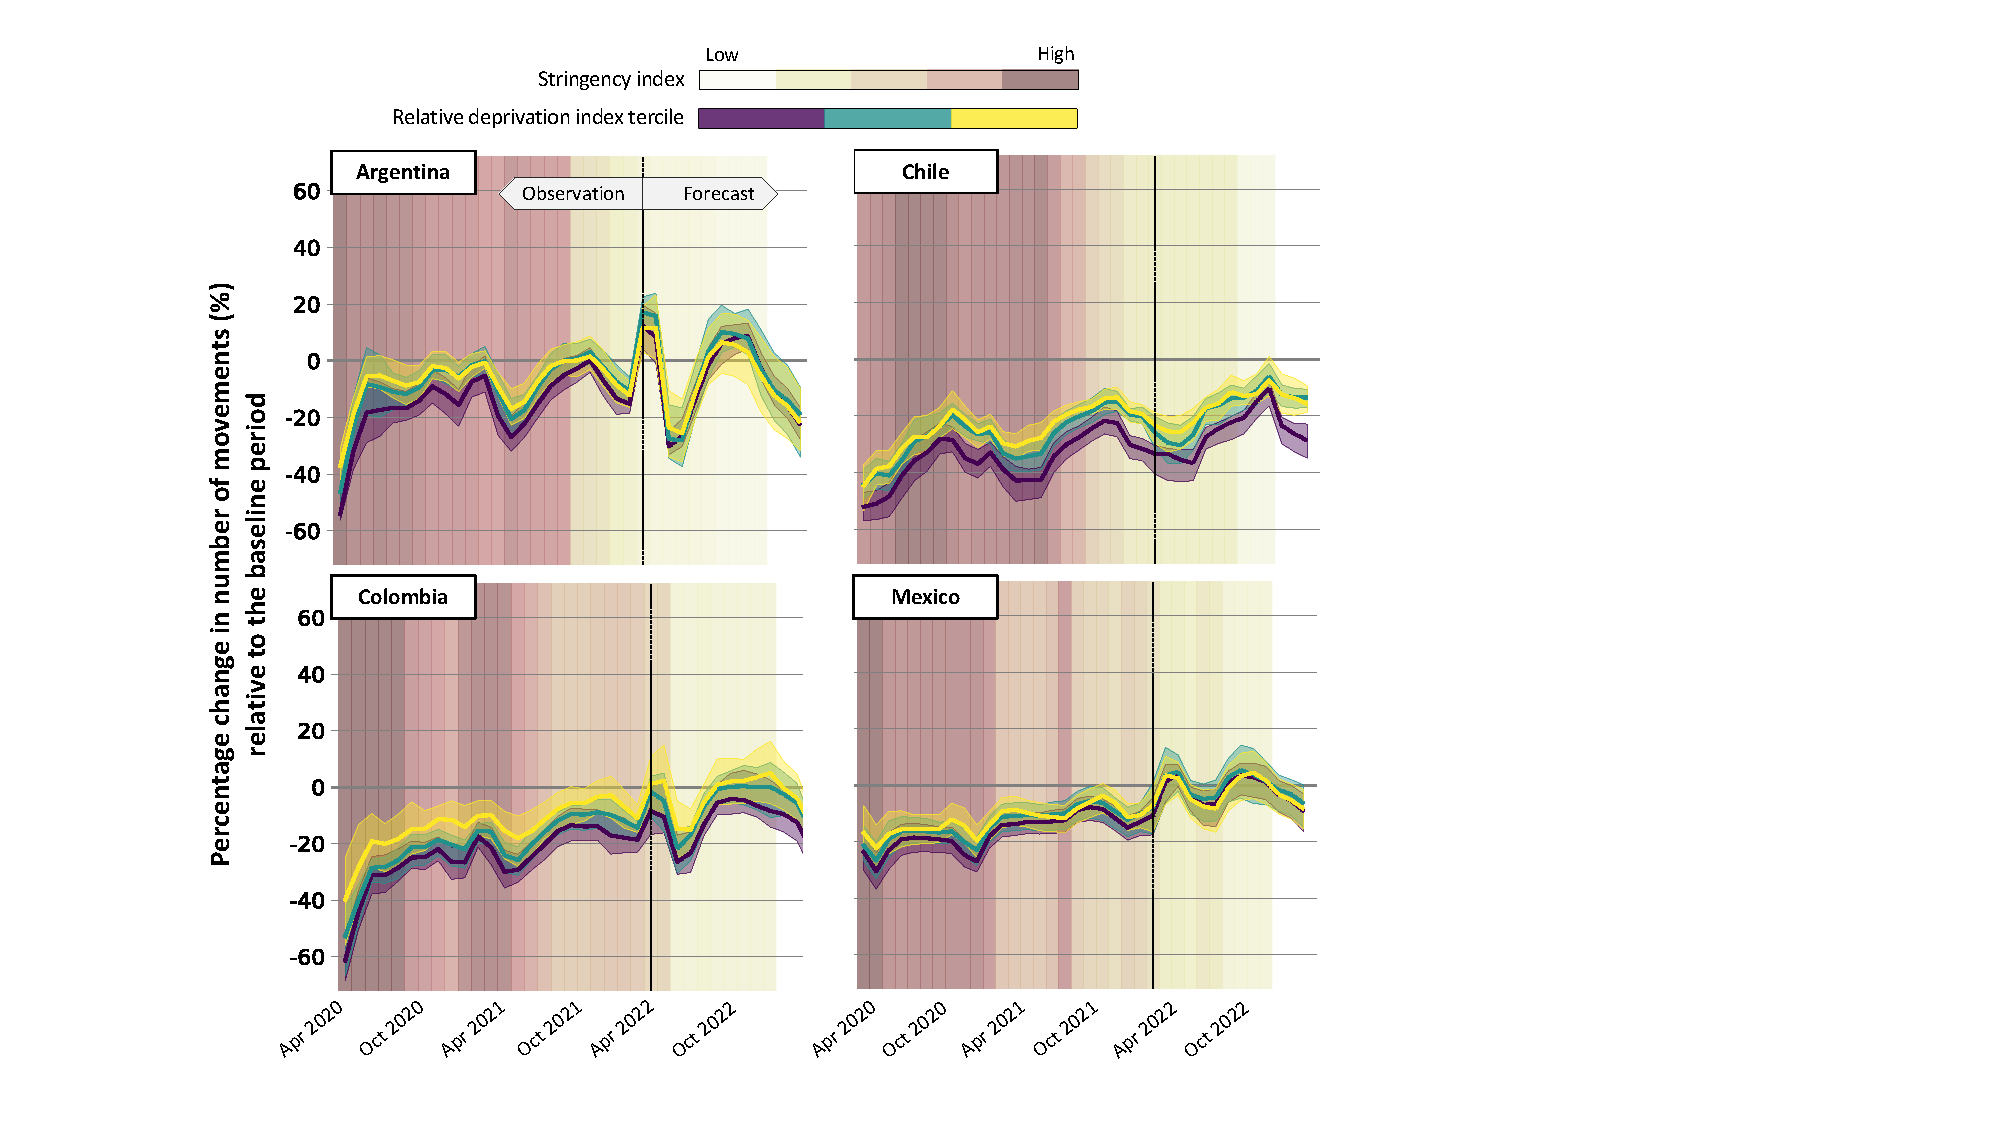
\includegraphics{figures/prediction-rdi-band.pdf}

}

\caption{Patterns of recovery for urban mobility in administrative units
from Argentina, Chile, Colombia and Mexico.}

\end{figure}

Generally, there was a drop in the levels of mobility with respect to
the baseline period in all four countries. This drop was especially
large for Argentina, Chile and Colombia, with Mexico displaying a
smaller decrease in the percentage change in the number of movements
with respect to the baseline. Following the initial drop in mobility,
all four countries evolve towards the recovery of baseline levels of
mobility, with a generally increasing trend. There are, however,
fluctuations from the general trend which manifest differently for each
country. These fluctuations mirror each other in the case of Argentina
and Colombia, where urban mobility sharply bounces back closer to
pre-pandemic levels around July of 2020. Chile and Mexico display more
progressive patterns of recovery, although Chile never reaches baseline
levels. These fluctuations are unique to each country and can be
attributed to local factors such as the effects of seasonality or the
different stringency measures imposed by the national governments during
the pandemic.

From Figure 2, we observe that there is a consistent tendency in how
administrative units with varying levels of deprivation were affected by
the pandemic. For all four countries, we observe that the administrative
units in the most deprived tercile are the ones that experienced the
smallest loss in levels of mobility at the beginning of the pandemic.
Differences in the levels of mobility across relative deprivation
terciles diminish with time. Argentina and Chile stand out as the
countries with the largest differences in mobility levels for different
relative deprivation terciles.

\hypertarget{the-most-deprived-areas-experienced-the-smallest-drop-in-mobility-relative-to-pre-pandemic-levels}{%
\subsection{The most deprived areas experienced the smallest drop in
mobility relative to pre-pandemic
levels}\label{the-most-deprived-areas-experienced-the-smallest-drop-in-mobility-relative-to-pre-pandemic-levels}}

In this section we explore further the role of socioeconomic deprivation
in the evolution of the levels of urban mobility. For a given point in
time (i.e.~a month), we start by considering the relationship between
the percentage change in the number of movements relative to the
pre-pandemic baseline period and the average RDI, at the administrative
unit level. We assume that this relationship is linear and we use a
linear regression to estimate the slope and intercept characterising the
line of best fit. This is shown for April 2020 and March 2022 in the
right-hand side panels of Figure 3. After obtaining the slope and
intercept for every month, we are able to plot the evolution of these
parameters for both the observed and forecasted data, as displayed on
the left-hand-side panels of the same Figure.

\begin{figure}

{\centering 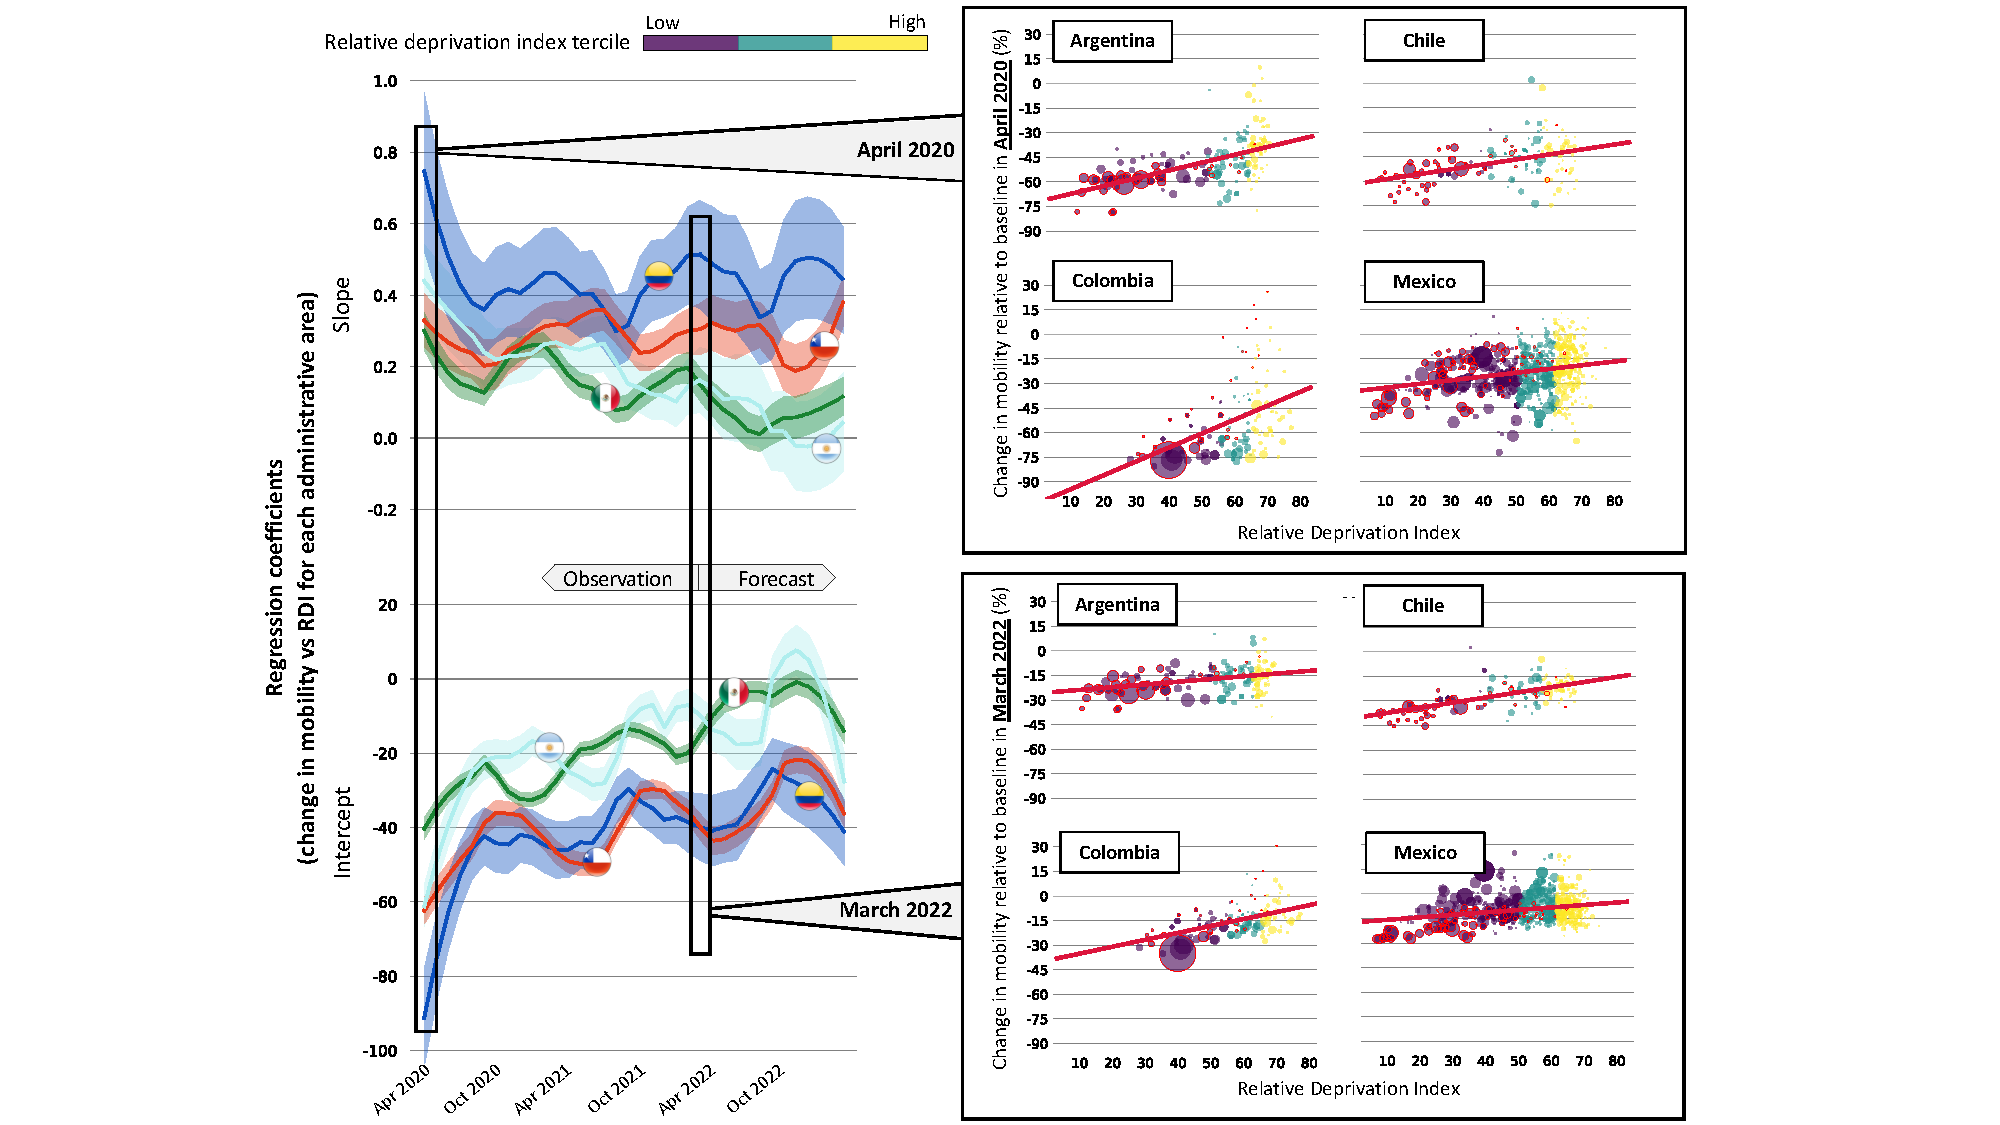
\includegraphics{figures/regression-evo-nobackground.pdf}

}

\caption{Evolution of the parameters characterising the relationship
between relative deprivation index and the percentage change in the
number of movements relative to the pre-pandemic baseline level of
mobility.}

\end{figure}

We find patterns in the evolution of the estimated parameters that
characterise the relationship between the levels of urban mobility and
RDI. In Argentina, Colombia and Mexico, we observe that the slope of
this relationship evolves to become smaller over time. The tendency is
not apparent in Chile, where the slope of the relationship remains
approximately the same over time despite the temporary fluctuations. The
slope captures the extent of differences in the level of urban mobility
across administrative units with varying levels of socioeconomic
deprivation. It can therefore be regarded as a measure of inequality in
mobility patterns across socioeconomic groups. A slope equal to zero
would mean that all administrative units display the same level of
mobility regardless of their average RDI. Given the patterns observed in
Argentina, Colombia and Mexico, we find that at the beginning of the
pandemic there were notable inequalities between socioeconomic groups in
terms of the levels of urban mobility. While it has taken more than two
years for Argentina and Mexico to close the gap (their slope is close to
zero from spring 2022), inequalities persist in Chile and Colombia as of
March 2023.

The intercept of the relationship displays stronger patterns, which are
consistent across the four countries. The intercept estimates the urban
mobility levels that would be observed in administrative units where the
RDI is zero. The intercept was below the baseline level at the early
stages of the pandemic. As observed in Figure 3, while there are some
differences between countries in the evolution of the intercept, the
general tendency is for the intercept to increase. While Argentina and
Mexico reach values that are closer to the baseline towards the end of
the forecast period, the intercept for Chile and Colombia remains lower.
Therefore, if there were areas with no socioeconomic deprivation, we
would have seen a recovery in the levels of mobility, especially in
Argentina and Mexico

\hypertarget{sec-discussion}{%
\section{Discussion}\label{sec-discussion}}

Using location data from Meta-Facebook users, our study aimed to examine
the evolution of patterns of mobility across socioeconomic groups in
functional urban areas from Argentina, Chile, Colombia and Mexico from
April 2020 to March 2023, following the COVID-19 pandemic. We found a
systematic drop in the number of population movements in April 2020,
with the largest reductions observed in the most affluent administrative
units within functional urban areas (FUAs) from Argentina, Chile and
Colombia. While mobility rebounded closer to pre-pandemic levels
approximately two years later, when COVID-19 restrictions eased, the
number of movements remained below pre-pandemic in Chile. Furthermore,
we found that at the beginning of the pandemic there were inequalities
between socioeconomic groups in terms of the levels of urban mobility.
While it has taken more than two years for Argentina and Mexico to
gradually reduce gap, inequalities persist as of March 2023, especially
in Chile and Colombia according to our estimated data.

We focused the analysis on short-distance movements in urban areas,
especifically those covering 70 km or less. These journeys are typically
considered to represent local and routine mobility (Owen and Green 1992)
. However, due to the characteristics of the Meta-Facebook movement
data, we are unable to distinguish the purpose of these short-distance
movements. Hence, some of our data could be capturing journeys that
involve a permanent change of place of residence. Our work therefore
motivates the need to answer questions regarding the validity of digital
footprint data for the analysis of human mobility. Further research
should focus on inferring more specific information about the nature of
the journeys, following similar approaches to those proposed by
Cabrera-Arnau et al. (2023), and quantifying the extent to which the
digital footprint data mirrors the true mobility patterns.

Conducting research on urban mobility using digital footprint data is
not straightforward, due to the challenges in accessing and working with
unstructured data sets which are often subject to biases and statistical
representation issues. These biases often arise from inequalities in
access and usage of digital technologies across demographic groups (Rowe
2023). Despite these challenges, the data and analysis that we used for
this work provide evidence for non-trivial patterns that are consistent
across four countries in Latin America and with other parts of the
world. Our findings highlight the dynamic interplay between
socioeconomic status and urban mobility, and shall be used to motivate
and inform the public debate regarding the deep societal consequences of
urban mobility disparities on the wider socioeconomic landscape of Latin
American countries.

In conclusion, we argue that this work goes beyond the analysis of
specific patterns by demonstrating the potential of digital footprint
data for policy-relevant research on human mobility at an unprecedented
level of spatiotemporal granularity. While we have seen a rise in
initiatives to improve data services and methodological frameworks to
facilitate the use of digital footprint data for social good, progress
is still limited, especially in some parts of the world including Latin
America. It is in the hands of governments and public organisations to
prioritise the maximisation the societal benefits that digital footprint
data has to offer. This includes engaging in activities such as building
strategic partnerships with commercial data-holders and academic
institutions to establish a unified framework for the use of digital
footprint data in policy and research. In particular, we call for the
creation of resources like those developed by the European Commission
Joint Research Centre (Commission et al. 2022) and the UN Statistics
Division (Division 2019), which identify sources of non-traditional data
and set methodological protocols for incorporating mobile phone data
into official mobility statistics. While current resources tend to have
a global reach, we advocate for more tailored local initiatives that
acknowledge disparities in regional data availability and adoption of
digital technologies.

\hypertarget{sec-methods}{%
\section{Methods}\label{sec-methods}}

\hypertarget{meta-facebook-movement-data}{%
\subsection{Meta-Facebook movement
data}\label{meta-facebook-movement-data}}

To capture population movements, we used anonymised aggregate mobile
phone location data from Meta users for Argentina, Colombia, Chile and
Mexico, covering a 24-month period from April 2020 to March 2022. We
used the dataset Facebook Movements created by Meta and accessed through
their Data for Good Initiative (\url{https://dataforgood.facebook.com}).
The data are built from Facebook app users who have the location
services setting turned on on their smartphone. Prior to releasing the
datasets, Meta ensures privacy and anonymity by removing personal
information and applying privacy-preserving techniques (Maas et al.
2019). Small-count dropping is one of these techniques. A data entry is
removed if the population or movement count for an area is lower than
10. The removal of small counts may mean that population counts in small
sparsely populated areas are not captured. A second technique consists
in adding a small undisclosed amount of random noise to ensure that it
is not possible to ascertain precise, true counts for sparsely populated
locations. Third, spatial smoothing using inverse distance-weighted
averaging is also applied is applied to produce a smooth population
count surface. The Facebook Movements dataset offers information on the
total number of Facebook users moving between and within spatial units
in the form of origin-destination matrices. The data is temporally
aggregated into three daily 8-hour time windows (i.e.~00:00-08:00,
08:00-16:00 and 16:00-00:00). The dataset includes a baseline capturing
the number of movements before COVID-19 based on a 45-day period ending
on March 10th 2020. The baseline is computed using an average for the
same time of the day and day of the week in the period preceding March
10th. For instance, the baseline for Monday 00:00-08:00 time window is
obtained by averaging over data collected on Mondays from 00:00 to 8:00
for the 45-day period. Details about the baseline can be found in (Maas
et al. 2019). The Bing Maps Tile System developed by Microsoft
(Microsoft) is used a spatial framework to organise the data. The Tile
System is a geospatial indexing system that partitions the world into
tile cells in a hierarchical way, comprising 23 different levels of
detail (Microsoft). At the lowest level of detail (Level 1), the world
is divided into four tiles with a coarse spatial resolution. At each
successive level, the resolution increases by a factor of two. The data
that we used are spatially aggregated into Bing tile levels 13. That is
about 4.9 x 4.9km at the Equator (Maas et al. 2019).

\hypertarget{spatiotemporal-data-aggregation}{%
\subsection{Spatiotemporal data
aggregation}\label{spatiotemporal-data-aggregation}}

Since the focus of this work is on urban mobility, we focus the analysis
on Functional Urban Areas (FUAs), defined by the Global Human Settlement
Layer (GHSL). The spatial extent of the FUAs is often large and may
include several towns and neighbourhoods displaying a variety of
socioeconomic characteristics, hence using FUAs as the spatial units of
aggregation would considerably mask the heterogeneity in the mobility
patterns. While the original unit of aggregation for the movement data,
i.e.~the tiles from the Bing Maps Tile System, offers the highest degree
of spatial granularity available, the interpretation of findings from an
analysis based on administrative units is often more valuable. For this
reason, we perform a spatial join to aggregate the movement data into
administrative units at the GADM level 2 or 3. Only flows of people
starting or ending within the boundaries of a FUA are considered.

While the original movement data is originally aggregated into 8-hour
windows, this resolution is too fine for our analysis. Since the
analysis is focused on the longer-term evolution of patterns of urban
mobility, we aggregate the movement data by month.

In our analysis, we use the Relative Deprivation Index (RDI) as a
measure of socioeocnomic deprivation. The RDI data is made available via
NASA's Socioeconomic Data and Applications Centre (SEDAC), with a
spatial resolution of 1km pixels. We perform a spatial join of the
gridded data and the administrative units and compute the average RDI
within each of these administrative units.

\hypertarget{time-series-analysis}{%
\subsection{Time series analysis}\label{time-series-analysis}}

For the countries included in the analysis, the movement data is
available until March 2022. In order to gain a better understanding of
the recovery trends after the pandemic, we generate a 12-month forecast
up to March 2023. This is done using Prophet (Taylor and Letham 2017), a
procedure developed by Meta's Core Data Science team to forecast time
series data based on an additive model. Prophet stands out from other
forecasting methods due to its ability to capture recurring seasonal
trends inherent in mobility data, such as fluctuations during holidays,
or changes in the general trend due to the impact of particular
circumstances, such as the COVID-19 pandemic. It is particularly
intuitive to use compared to other models due to its automated
trend-detection capabilities, making it accessible to users with no
expertise on the underlying model, while being robust to missing data
and outliers. For the analysis in this paper, yearly seasonality effects
are included as they yield the most realistic predictions.

Figures 2 and 3 have been created by removing statistical outliers. We
define these as the administrative units which, at any given month, have
a z-score greater than 4 for the percentage change in the number of
movements. Furthermore, a Savitzky-Golay filter is applied to smooth the
time series data, using a length of 4 units for the filter window and
order 2 polynomials to fit the samples.

\hypertarget{references}{%
\section*{References}\label{references}}
\addcontentsline{toc}{section}{References}

\hypertarget{refs}{}
\begin{CSLReferences}{1}{0}
\leavevmode\vadjust pre{\hypertarget{ref-LaurenAlexander15}{}}%
Alexander, Lauren, Shan Jiang, Mikel Murga, and Marta C. González. 2015.
{``Origin--Destination Trips by Purpose and Time of Day Inferred from
Mobile Phone Data.''} \emph{Transportation Research Part C: Emerging
Technologies} 58: 240--50.
https://doi.org/\url{https://doi.org/10.1016/j.trc.2015.02.018}.

\leavevmode\vadjust pre{\hypertarget{ref-Cabrera-Arnau2023}{}}%
Cabrera-Arnau, Carmen, Chen Zhong, Michael Batty, Ricardo Silva, and
Soong Moon Kang. 2023. {``Inferring Urban Polycentricity from the
Variability in Human Mobility Patterns.''} \emph{Scientific Reports} 13
(1): 5751. \url{https://doi.org/10.1038/s41598-023-33003-7}.

\leavevmode\vadjust pre{\hypertarget{ref-RDI2022}{}}%
Columbia University, Center for International Earth Science Information
Network. CIESIN. 2022. {``Global Gridded Relative Deprivation Index
(GRDI), Version 1.''} Palisades, New York: NASA Socioeconomic Data;
Applications Center (SEDAC). \url{https://doi.org/10.7927/3xxe-ap97}.

\leavevmode\vadjust pre{\hypertarget{ref-ECJRC22}{}}%
Commission, European, Joint Research Centre, C Bosco, S
Grubanov-Boskovic, S Iacus, U Minora, F Sermi, and S Spyratos. 2022.
\emph{Data Innovation in Demography, Migration and Human Mobility}.
Publications Office of the European Union.
\url{https://doi.org/doi/10.2760/027157}.

\leavevmode\vadjust pre{\hypertarget{ref-UNSD}{}}%
Division, United Nations Statistical. 2019. {``Handbook on the Use of
Mobile Phone Data for Official Statistics.''}

\leavevmode\vadjust pre{\hypertarget{ref-GADM24}{}}%
GADM. 2024. {``GADM Maps and Data.''}

\leavevmode\vadjust pre{\hypertarget{ref-Maas19}{}}%
Maas, P., S. Iyer, A. Gros, W. Park, L. McGorman, C. Nayak, and P. A.
Dow. 2019. {``Facebook Disaster Maps: Aggregate Insights for Crisis
Response and Recovery.''} In \emph{16th International Conference on
Information Systems for Crisis Response and Management}, 836--47.

\leavevmode\vadjust pre{\hypertarget{ref-MengChuishi17}{}}%
Meng, Chuishi, Yu Cui, Qing He, Lu Su, and Jing Gao. 2017. {``Travel
Purpose Inference with GPS Trajectories, POIs, and Geo-Tagged Social
Media Data.''} In \emph{2017 IEEE International Conference on Big Data
(Big Data)}, 1319--24.
\url{https://doi.org/10.1109/BigData.2017.8258062}.

\leavevmode\vadjust pre{\hypertarget{ref-NiluferSariAslam21}{}}%
Nilufer Sari Aslam, Tao Cheng, Mohamed R. Ibrahim, and Yang Zhang. 2021.
{``ActivityNET: Neural Networks to Predict Public Transport Trip
Purposes from Individual Smart Card Data and POIs.''} \emph{Geo-Spatial
Information Science} 24 (4): 711--21.
\url{https://doi.org/10.1080/10095020.2021.1985943}.

\leavevmode\vadjust pre{\hypertarget{ref-owen1992migration}{}}%
Owen, D., and A. Green. 1992. {``Migration Patterns and Trends.''} In
\emph{Migration Processes and Patterns: Research Progress and
Prospects}, edited by T. Champion and T. Fielding. Belhaven Press.

\leavevmode\vadjust pre{\hypertarget{ref-RoweBigData23}{}}%
Rowe, Francisco. 2023. {``9.: Big Data.''} In \emph{Concise Encyclopedia
of Human Geography}, 42--47. Cheltenham, UK: Edward Elgar Publishing.
\url{https://doi.org/10.4337/9781800883499.ch09}.

\leavevmode\vadjust pre{\hypertarget{ref-roweCalafiore2022}{}}%
Rowe, Francisco, Alessia Calafiore, Daniel Arribas-Bel, Krasen
Samardzhiev, and Martin Fleischmann. 2022. {``Urban Exodus?
Understanding Human Mobility in Britain During the COVID-19 Pandemic
Using Facebook Data.''} \url{https://doi.org/10.48550/ARXIV.2206.03272}.

\leavevmode\vadjust pre{\hypertarget{ref-GHSL19}{}}%
Schiavina M., Maffenini L., Moreno-Monroy A. 2019. {``GHS-FUA R2019A -
GHS Functional Urban Areas, Derived from GHS-UCDB R2019A, (2015),
R2019A.''} European Commission, Joint Research Centre (JRC).

\leavevmode\vadjust pre{\hypertarget{ref-prophet17}{}}%
Taylor, Sean J, and Benjamin Letham. 2017. {``Forecasting at Scale.''}
\emph{PeerJ Preprints} 5 (September): e3190v2.
\url{https://doi.org/10.7287/peerj.preprints.3190v2}.

\leavevmode\vadjust pre{\hypertarget{ref-wang2022}{}}%
Wang, Yikang, Chen Zhong, Qili Gao, and Carmen Cabrera-Arnau. 2022.
{``Understanding Internal Migration in the UK Before and During the
COVID-19 Pandemic Using Twitter Data.''} \emph{Urban Informatics} 1 (1).
\url{https://doi.org/10.1007/s44212-022-00018-w}.

\end{CSLReferences}



\end{document}
